\documentclass{article}
\usepackage{graphicx}
\usepackage{algorithm}
\usepackage{algpseudocode}
\usepackage{bookmark}
\usepackage{amsmath}
\graphicspath{ {images/} }
\bibliographystyle{unsrtnat}

% if you need to pass options to natbib, use, e.g.:
%     \PassOptionsToPackage{numbers, compress}{natbib}
% before loading neurips_2023


% ready for submission
\usepackage[preprint]{neurips_2023}


% to compile a preprint version, e.g., for submission to arXiv, add add the
% [preprint] option:
%     \usepackage[preprint]{neurips_2023}


% to compile a camera-ready version, add the [final] option, e.g.:
%     \usepackage[final]{neurips_2023}


% to avoid loading the natbib package, add option nonatbib:
%    \usepackage[nonatbib]{neurips_2023}


\usepackage[utf8]{inputenc} % allow utf-8 input
\usepackage[T1]{fontenc}    % use 8-bit T1 fonts
\usepackage{url}            % simple URL typesetting
\usepackage{booktabs}       % professional-quality tables
\usepackage{amsfonts}       % blackboard math symbols
\usepackage{nicefrac}       % compact symbols for 1/2, etc.
\usepackage{microtype}      % microtypography
\usepackage{xcolor}         % colors
\usepackage{hyperref}       % hyperlinks


\title{HERACLES to the Rescue: Hyperbolic Embeddings for Reconstruction and Analysis of CRISPR-Cas9 LineagES}

\author{%
  Gilad Turok\thanks{\url{https://gil2rok.github.io/}} \\
  Department of Computer Science\\
  Columbia University\\
  New York, New York 10025 \\
  \texttt{gt2453@columbia.edu} \\
}


\begin{document}
\maketitle


\begin{abstract}
  Tracking the fate of single cells is immensely important in contemporary biology. With the advent of CRISPR-Cas9 genome editing and high-throughout single-cell sequencing, this is now a reality. To that end, we present HERACLES, a novel phylogeny-reconstruction algorithm to recover the cell lineage of CRISPR-Cas9  experiments. HERACLES learns hyperbolic embeddings by maximizing a CRISPR-specific log-likelihood function, thus reconstructing the phylogenetic tree of interest while addressing the unique challenges of CRISPR-based lineage tracking. We provide early simulation experiments that demonstrate the efficacy of HERACLES, surpassing  current state-of-the-art algorithms. An implementation of HERACLES is available at \url{https://github.com/gil2rok/crispr-phylogeny}.
\end{abstract}


%%%%%%%%%%%%%%%%%%%%%%%%%%%%%%%%%%%%%%%%%%%%%%%%%%%%%%%%%%%%
\section{Introduction}
%%%%%%%%%%%%%%%%%%%%%%%%%%%%%%%%%%%%%%%%%%%%%%%%%%%%%%%%%%%%


The ability to track individual cells throughout biological processes has significant and immense potential, especially during regimes of cellular development or cancer. With the advent of CRISPR-Cas9 gene editing and single-cell sequencing technologies, we can now track the lineage of a particular cell by inserting a heritable \emph{casette} into its genome. Each casette contains multiple \emph{target sites} on which CRISPR-induced insertions and deletions (\emph{indels}) can occur and be passed down to its descendents. Many generations later, these casettes are sequenced and the indels at each target site are recorded, forming a \emph{character matrix}. With this character matrix, a phylogenetic algorithm attempts to reconstruct the original cell-lineage as a phylogenetic tree as in \ref{fig:problem_statement}. Using this method, biologists have uncovered unprecented insights into zebrafish \cite{McKenna2016} \cite{Raj2018}  and mouse development \cite{Kalhor2018} \cite{chan2019}, among other discoveries.

\begin{figure}[t]
  \label{fig:problem_statement}
  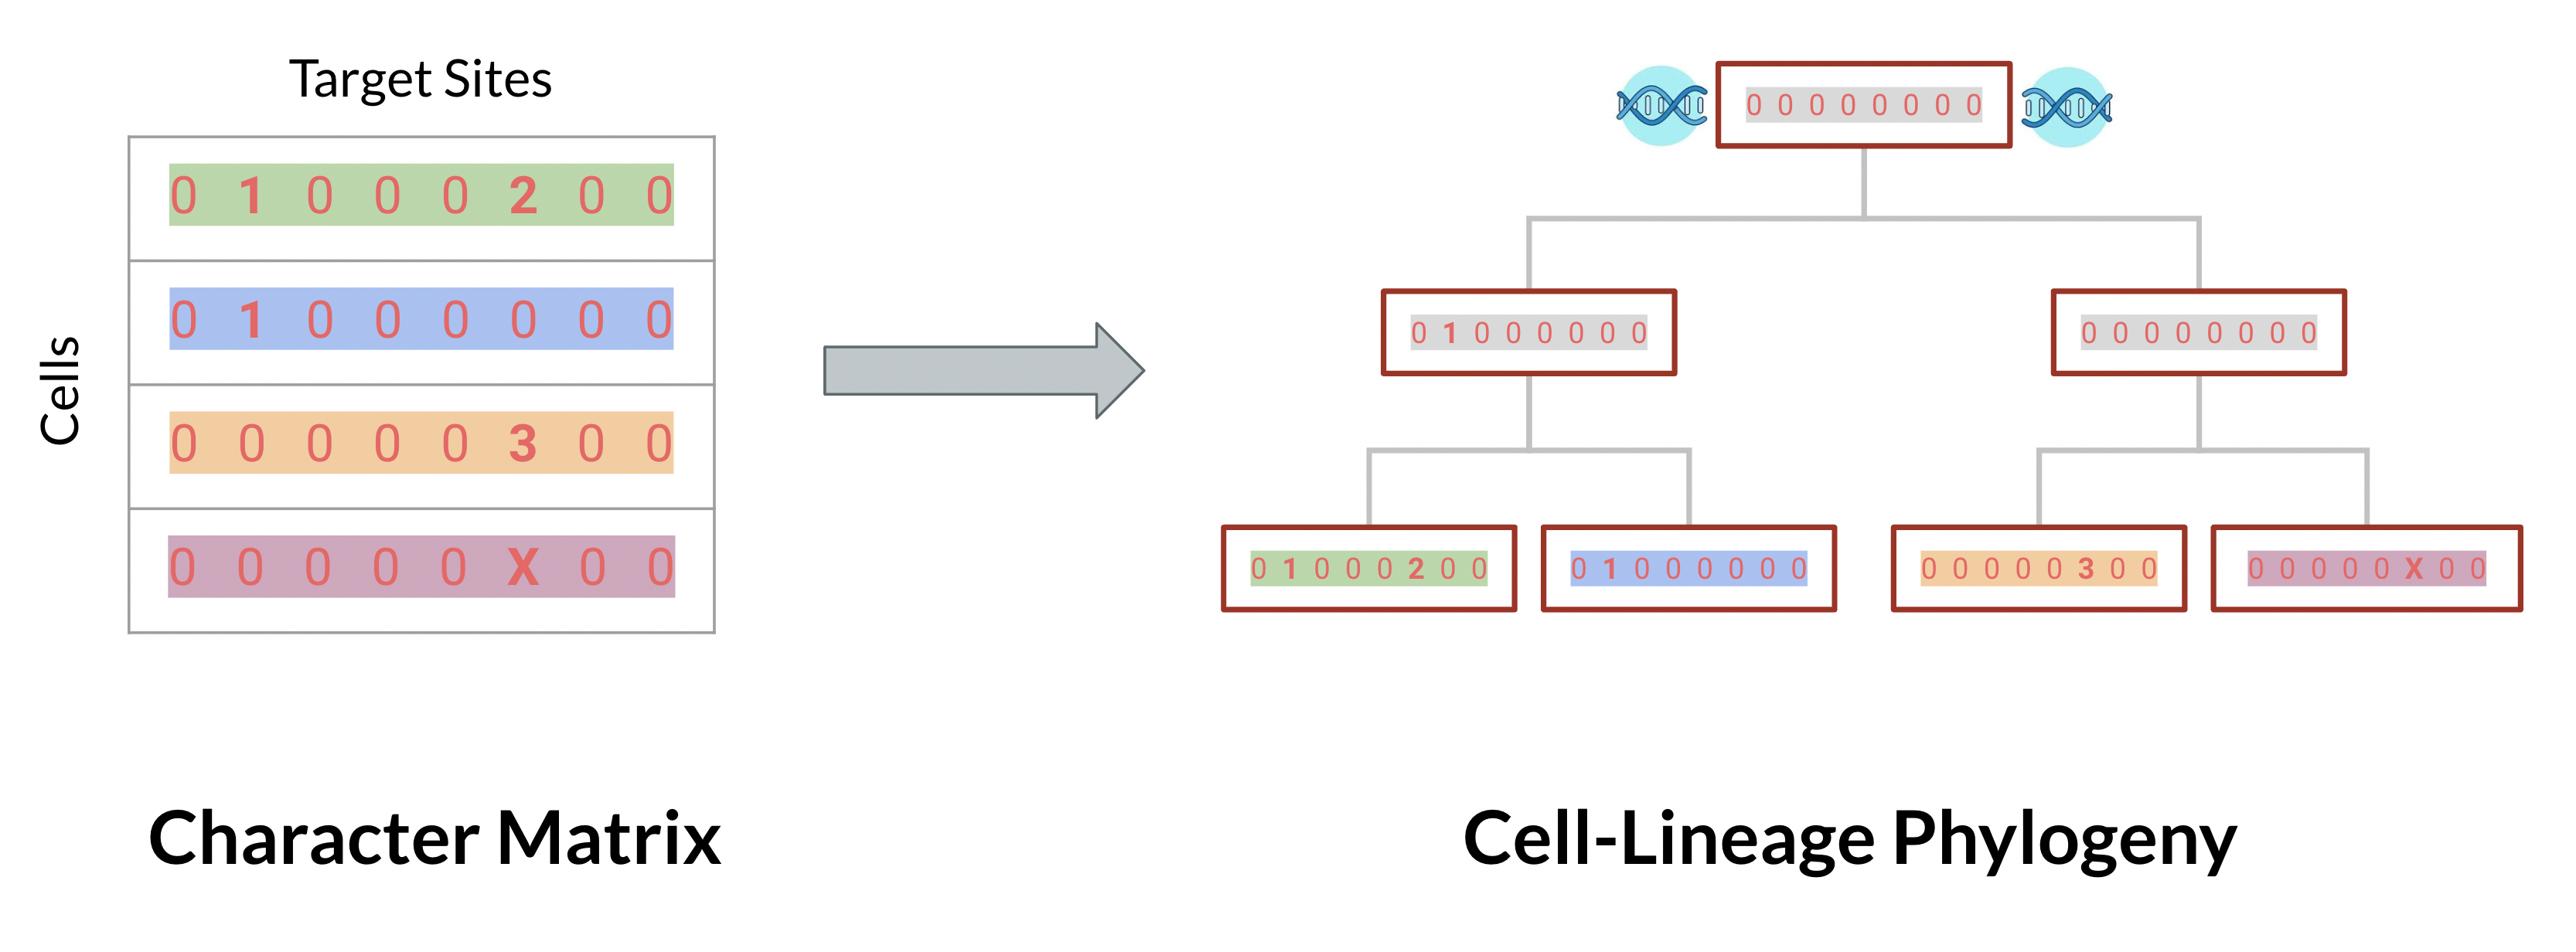
\includegraphics[width=\linewidth]{images/problem_statement.png}
  \caption{From a character matrix, HERACLES seeks to reconstruct the original cell-lineage as a phylogenetic tree.}
\end{figure}

Many phylogeny-reconstrution algorithms, however, are not well-suited for CRISPR-Cas9 cell-lineage data because of its (1) scale, (2) sequencing challenges, and (3) unique evolutionary model. As such, traditional algorithms -- such as Neighbor Joining \cite{saitou1987neighbor}, Weighbor \cite{bruno2000}, and Camin-Sokal \cite{camin1965method} -- may not perform well in this domain. These traditional algorithms are suited for a few samples, not tens of thousands of cells. This largely makes them computationally intractable for cell-lineage data. Furthermore, these algorithms are unable to handle the vast amounts of missing data that occur in single-cell-lineage tracing: missing data may be \emph{heritable} -- from large-scale CRISPR-induced deletions -- or \emph{stochastic} -- from incomplete capture of target sites during sequencing. Finally, these algorithms do not take into account the design of lineage tracers and the evolutionary stochastic models they induce. Unlike cannonical evolutionary models, lineage tracing experiments are time-irreversible such that once an edit is made, reversions to an unedited start or a different mutation are impossible.  Furthermore, in this setting the ancestral state, or root of the lineage tree, is known to be the unedited state; this information can be used to inform the construction of the phylogenetic tree. Thirdly, lineage tracing systems contain site-specific mutation rates that enable capturing evolutionary relationships at varying time-scales.

We aim to tackle these challenges by developing a novel phylogeny-reconstruction algorithm HERACLES: Hyperbolic Embeddings for Reconstruction and Analysis of CRISPR-Cas9 LineagES. HERACLES explicitly considers (1) different mutation rates at each target site, (2) non-uniform distributions over indels at each target site, and (3) time-irreversible evolutionary model of lineage tracing experiments. HERACLES broadly works by finding hyperbolic embeddings that accurately represent the phylogenetic tree of interest. First we identify the continous time Markov-chain that underlies the evolutionary process of the lineage tracing experiment. In this context, we construct a log-likelihood function that quantifies the fidelity of a candidate phylogenetic tree. Next, we embed the character matrix into hyperbolic space and use gradient-based optimization to find the embedding that maximizes the log-likelihood function. Finally, we reconstruct the phylogenetic tree from these hyperbolic embeddings. We provide early simulation experiments that demonstrate the efficacy of HERACLES.


%%%%%%%%%%%%%%%%%%%%%%%%%%%%%%%%%%%%%%%%%%%%%%%%%%%%%%%%%%%%
\section{Related Work}
%%%%%%%%%%%%%%%%%%%%%%%%%%%%%%%%%%%%%%%%%%%%%%%%%%%%%%%%%%%%


Previous work has been carried out in \cite{wilson2021learning} that reconstructs phylogentic trees with hyperbolic embeddings for homologous sequence data, generated under the Jukes-Cantor evolutionary model. They find that using hyperbolic embeddings outperforms many traditional phylogeny-reconstruction algorithms in a variety of simulated settings. This paper (similarly) reconstructs phylogenetic trees with hyperbolic embeddings but does so for the evolutionary model of CRISPR-Cas9 lineage tracing. Furthermore, \cite{jones2020inference} is the only work that directly tackles lineage tracing for CRISPR-Cas9. They propose three approaches: greedily optimizing for parsimony, finding a Steiner Tree with Integer Linear Programming (ILP), and a hybrid approach that combines the two. HERACLES can be viewed as a combination of these two works, learning hyperbolic embeddings for CRISPR-Cas9 lineage tracing experiments.


%%%%%%%%%%%%%%%%%%%%%%%%%%%%%%%%%%%%%%%%%%%%%%%%%%%%%%%%%%%%
\section{Methods}
%%%%%%%%%%%%%%%%%%%%%%%%%%%%%%%%%%%%%%%%%%%%%%%%%%%%%%%%%%%%


\subsection{Preliminaries}

\paragraph*{Character Matrix} Every row in the character matrix $C$ describes the casette for one of $N$ cells and each casette contains a variety of target sites. A target site $\sigma$ in cell $c$ can be unedited, mutated, or deleted -- although a variety of different mutations exists. Formally, let $\sigma_c \in \{0, 1, \ldots, M_\sigma, D \}$ where $0$ represents the unedited state, $1, \ldots, M_\sigma$ represent the different mutations, and $D$ represents a deletion.

\paragraph*{Transition Matrix} The accumulation of CRISPR-Cas9 induced edits at a given target site $\sigma$ evolves as a time-homogeneous continuous time Markov chain. This emits a row-stochastic matrix $P^\sigma$ that defines a time-homogeneous and time-irreversible model of mutation. This transition matrix $P^\sigma$ is target-site dependent but we will drop the explicit dependence on target site and just write $P$. For mutation states $a$ and $b$, the entry $P_{ab}(t)$ is the probability of transitioning from state $a$ to state $b$ in $t$ time steps.

\paragraph*{Infinitesimal Generator} As a continous time Markov chain, the probablity matrix $P$ is determined by its infinitesimal generator $Q$ by

\begin{equation}
  P_{ab}(t) = e^{t \cdot Q_{ab}}
\end{equation}

For each target site $\sigma$, the time to leave the unedited state is exponentially distributed with rate $\lambda=\lambda_{M \sigma} + \lambda_D$ for the site-specific rate $\lambda_{M \sigma}$ and the (small) deletion rate $\lambda_D$. Given that a transition occurs to some other character state, the transition to the observed character state, $s$, occurs with probability $p_{\phi_\sigma s}$ such that $\sum_{i \in M_\sigma} p_{\phi_\sigma i} = 1$. (Note $P$ represents the transition matrix while $p$ represents the indel distribution.)

The site-specific mutation rates $\lambda_{M \sigma}$, deletion rate $\lambda_D$, and indel distribution $p$ can be determined by sensor screens performed a priori or inferred directly from the character matrix.

A toy example of the infinitesimal generator $Q$ is found in the appendix \ref{fig:Q}.

\paragraph*{Log-likelihood Function} Consider $\sigma_i$ and $\sigma_j$, a specific target site $\sigma$ for cells $i$ and $j$ respectively. Because CRISPR-Cas9 lineage tracing is time-irreversible, we must consider a common ancestor $a$ and examine the time it takes from $a$ to evolve into states $\sigma_i$ and $\sigma_j$. We make the simplifying assumption that the ancestral state $a$ is equidistant to both states $\sigma_i$ and $\sigma_j$. 

Thus we compute the likelihood of the two cells being separated by an evolutionary distance of $t$ time units as:

\begin{equation}
  \mathcal{L}_{ij}^P (t) = \prod_{\textrm{site } \sigma} \sum_{a \in A(\sigma_i, \sigma_j)} \pi_a \; P_{a \sigma_i}(t/2) \; P_{a \sigma_j}(t/2).
\end{equation}

Here $\pi_a$ is the prior probability of being in an ancestral state $a$, $P_{a \sigma_i}$ is the probability of transitioning from $a$ to $\sigma_i$ in $t/2$ time units, and $P_{a \sigma_j}$ is the probability of transitioning from $a$ to $\sigma_j$ in $t/2$ time units. Furthermore, we iterate over all target sites $\sigma$ and over all feasible ancestors $A(\sigma_i, \sigma_j)$ for cells $i$ and $j$ at site $\sigma$.

The ancestral priors $\pi_a$ are learned from Felstenstein's algorithm \cite{felsenstein1973maximum}. The feasible ancestors $A(\sigma_i, \sigma_j)$ are constrainted to a limited set of states, including the unedited state $0$ and the least common ancestor of $\sigma_i$ and $\sigma_j$. We compute the set of feasible ancestors as

\begin{equation}
  A(\sigma_i, \sigma_j) = \begin{cases}
    \{0, \sigma_i \} & \textrm{\quad if } \sigma_i = \sigma_j \\
    \{0 \} & \textrm{\quad if } \sigma_i \neq \sigma_j \\
  \end{cases}
\end{equation}

Thus the log-likelihood function ultimately quanitifes the fidelity of cell $i$ and cell $j$ being separated by an evolutionary distance of $t$ time units, as informed by our assumptions about the transition matrix $P$. Also, in practice we compute the log-likelihood to avoid numerical issues.

\subsection{The HERACLES Algorithm}

The HERACLES algorithm consists of three steps: embedding the character matrix into hyperbolic space, optimizing the hyperbolic embeddings with respect to the log-likelihood function, and recovering a phylogenetic tree from the optimized hyperbolic embeddings. HERACLES is presented in its entirety in \ref{alg:heracles} and we now describe each step in detail.

\begin{algorithm}[t]
  \caption{HERACLES}
  \label{alg:heracles}
  \begin{algorithmic}
  \Require Character matrix $C$, Transition matrix $P$
  \State $D = $HammingDist$(C)$ \Comment{Pairwise distance matrix}
  \State $T = $TreeReconstruction$(D)$ \Comment{Reconstructed tree}
  \State $X = $SarkarsConstruction$(T)$ \Comment{Initial hyperbolic embedding}
  \\
  \While{not converged}
  \State \textbf{for} $i = 1, \dots, N$ \textbf{do}
  \State \quad $L = \sum_{j} \log \mathcal{L}_{ij}^P\left(d(x_i, x_j) \right)$ \Comment{Log-likelihood for cell $i$}
  \State \quad $x_i \leftarrow$ RiemmanianAdam$(x_i, \nabla_{x_i} L)$ \Comment{Gradient Update}
  \State \textbf{end for}
  \EndWhile
  \\
  \State $D^\prime = $GeodesicDist$(X)$ \Comment {Pairwise distance matrix}
  \State $T^\prime = $TreeReconstruction$(X)$ \Comment{Reconstructed tree}
  \end{algorithmic}
\end{algorithm}

\paragraph*{Embedding the Character Matrix into Hyperbolic Space} To embed the character matrix $C$ into hyperbolic space, we first compute a pairwise distance matrix $D$ with the Hamming distance between each pair of cells. We then use a tree reconstruction algorithm -- such as Neighbor Joining -- to construct an intial phylogenetic tree $T$. Finally, we use a generalization of Sarkar's construction \cite{sarkar2012low} \cite{sala2018representation} to isometrically embed the tree into hyperbolic space as a point cloud, serving as the initial embedding $X$ to be optimized.

\paragraph*{Optimizing the Hyperbolic Embeddings} We iteravely optimize the hyperbolic embeddings $X$ for one cell-embedding ($x_i$) at a time. For each cell $i$, we sum over a minibatch of cells $j$ and compute the log-likelihood:

\begin{align}
  \label{eq:log-likelihood}
  L &= \sum_{j} \log \mathcal{L}_{ij}^P \left( d(x_i, x_j) \right) \\
  &= \sum_{j} \log \left[ \prod_{\textrm{sites } \sigma} \sum_{a \in A(\sigma_i, \sigma_j)} \pi_a \; P_{a \sigma_i} \left( \frac{ d(x_i, x_j)}{2} \right) \;   P_{a \sigma_j} \left( \frac{ d(x_i, x_j)}{2} \right) \right].
\end{align}

Note that we set $t=d(x_i, x_j)$ such that instead of $\sigma_i$ and $\sigma_j$ being seperated by $t$ time units, we use the geodesic distance $d(x_i, x_j)$ between the embeddings $x_i$ and $x_j$.

After computing the log-likelihood, we update the embedding $x_i$ of cell $i$ with the Riemannian Adam optimizer \cite{becigneul2018riemannian}. Riemannian Adam is a modified Adam optimizer \cite{kingma2014adam} that ensures the update remains on the manifold of hyperbolic space. As we iterate through the $N$ cells, we updated the embedding $X$ iteratively, repeating this process until some convergence criteria is met.

\paragraph*{Recovering the Phylogenetic Tree} Once the hyperbolic embeddings $X$ have converged, we compute a pairwise distance matrix $D^\prime$ with the geodesic distance between each pair of cells. We then use a tree reconstruction algorithm -- such as Neighbor Joining -- to construct a phylogenetic tree $T^\prime$. The reconstructed tree of cell-lineages, $T^\prime$, is the final output of the HERACLES algorithm.


%%%%%%%%%%%%%%%%%%%%%%%%%%%%%%%%%%%%%%%%%%%%%%%%%%%%%%%%%%%%
\section{Experiments and Discussion}
%%%%%%%%%%%%%%%%%%%%%%%%%%%%%%%%%%%%%%%%%%%%%%%%%%%%%%%%%%%%


To test HERACLES, we simulated a ground truth phylogeny with a birth death process and then overlayed casettes on this tree topology. We where then able to compare the true tree to an estimated tree with the triplets correct metric \cite{sand2013practical}, in which higher is better. In these experiments, we investigate the performance of HERACLES, the Cassiopeia greedy algorithm, and the Cassiopeia ILP algorithm. Extra figures are linked to in the appendix.

In small simulations of $N=20$ cells, HERACLES learns good hyperbolic embeddings: the log-likelihood and triplets correct metric both increase \ref{fig:loss_20} \ref{fig:tc_20}. Furthermore, HERACLES outperforms both state-of-the-art Cassiopeia algorithms \ref{tab:results}.

In larger simulations of $N=1000$ cells, HERACLES again outperforms both state-of-the-art Cassiopeia algorithms \ref{tab:results}. However, in this setting, HERACLES is unable to improve the initial hyperbolic embeddings as the log-likelihood and triplets correct metric fluctuate stochastically but do not increase \ref{fig:loss_1000} \ref{fig:tc_1000}. This suggests that the initial embedding scheme into hyperbolic space works well but the gradient updates from RiemannianAdam do not.


\begin{table}[t]
  \label{tab:results}
  \begin{center}
    \begin{tabular}{||c c c c||} 
      \hline
        \\  & HERACLES &  Cassiopeia ILP & Cassiopeia Greedy  \\ 
      \hline\hline
      $20$ cells & \textbf{0.465}  & 0.457 & 0.310 \\ 
      \hline
      $1000$ cells & \textbf{0.260} & 0.049 & 0.10 \\
      \hline
    \end{tabular}
  \end{center}
  \caption{Results of HERACLES, Cassiopeia ILP and Cassiopeia Greedy on simulated data.}
\end{table}


%%%%%%%%%%%%%%%%%%%%%%%%%%%%%%%%%%%%%%%%%%%%%%%%%%%%%%%%%%%%
\section{Conclusion}
%%%%%%%%%%%%%%%%%%%%%%%%%%%%%%%%%%%%%%%%%%%%%%%%%%%%%%%%%%%%


In this paper we explored reconstructing cell-lineages of CRISP-Cas9 experiments. We introduced HERACLES, a novel algorithm that embeds a character matrix into hyperbolic space, improves the hyperbolic embeddings with RiemannianAdam, and then reconstructs the original phylogenetic tree. We showed that HERACLES outperforms state-of-the-art Cassiopeia algorithms on simulated data.

At the moment, HERACLEs benefits from the initial embedding but not from out gradient updates. However, it is remarkable that the initial embedding into hyperboloc space makes such a significant difference in the performance of HERACLES.

In future work, we plan to investigate HERACLES' performance in a much wider variety of simulated settings to ensure robust performance. We also plan to explore alternative embedding schemes for the initial embedding into hyperbolic space. Furthermore, we plan to extensively explore why HERACLES fails to improve the hyperbolic embeddings in larger simulations. Finally, we plan to apply HERACLES to real CRISP-Cas9 data.


%%%%%%%%%%%%%%%%%%%%%%%%%%%%%%%%%%%%%%%%%%%%%%%%%%%%%%%%%%%%
\bibliography{references}
%%%%%%%%%%%%%%%%%%%%%%%%%%%%%%%%%%%%%%%%%%%%%%%%%%%%%%%%%%%%

\section*{Appendix}

\subsection*{Infinitesimal Generator $Q$ for Toy Lineage Tracing Experiment}

\begin{figure}[h]
  \label{fig:Q}
  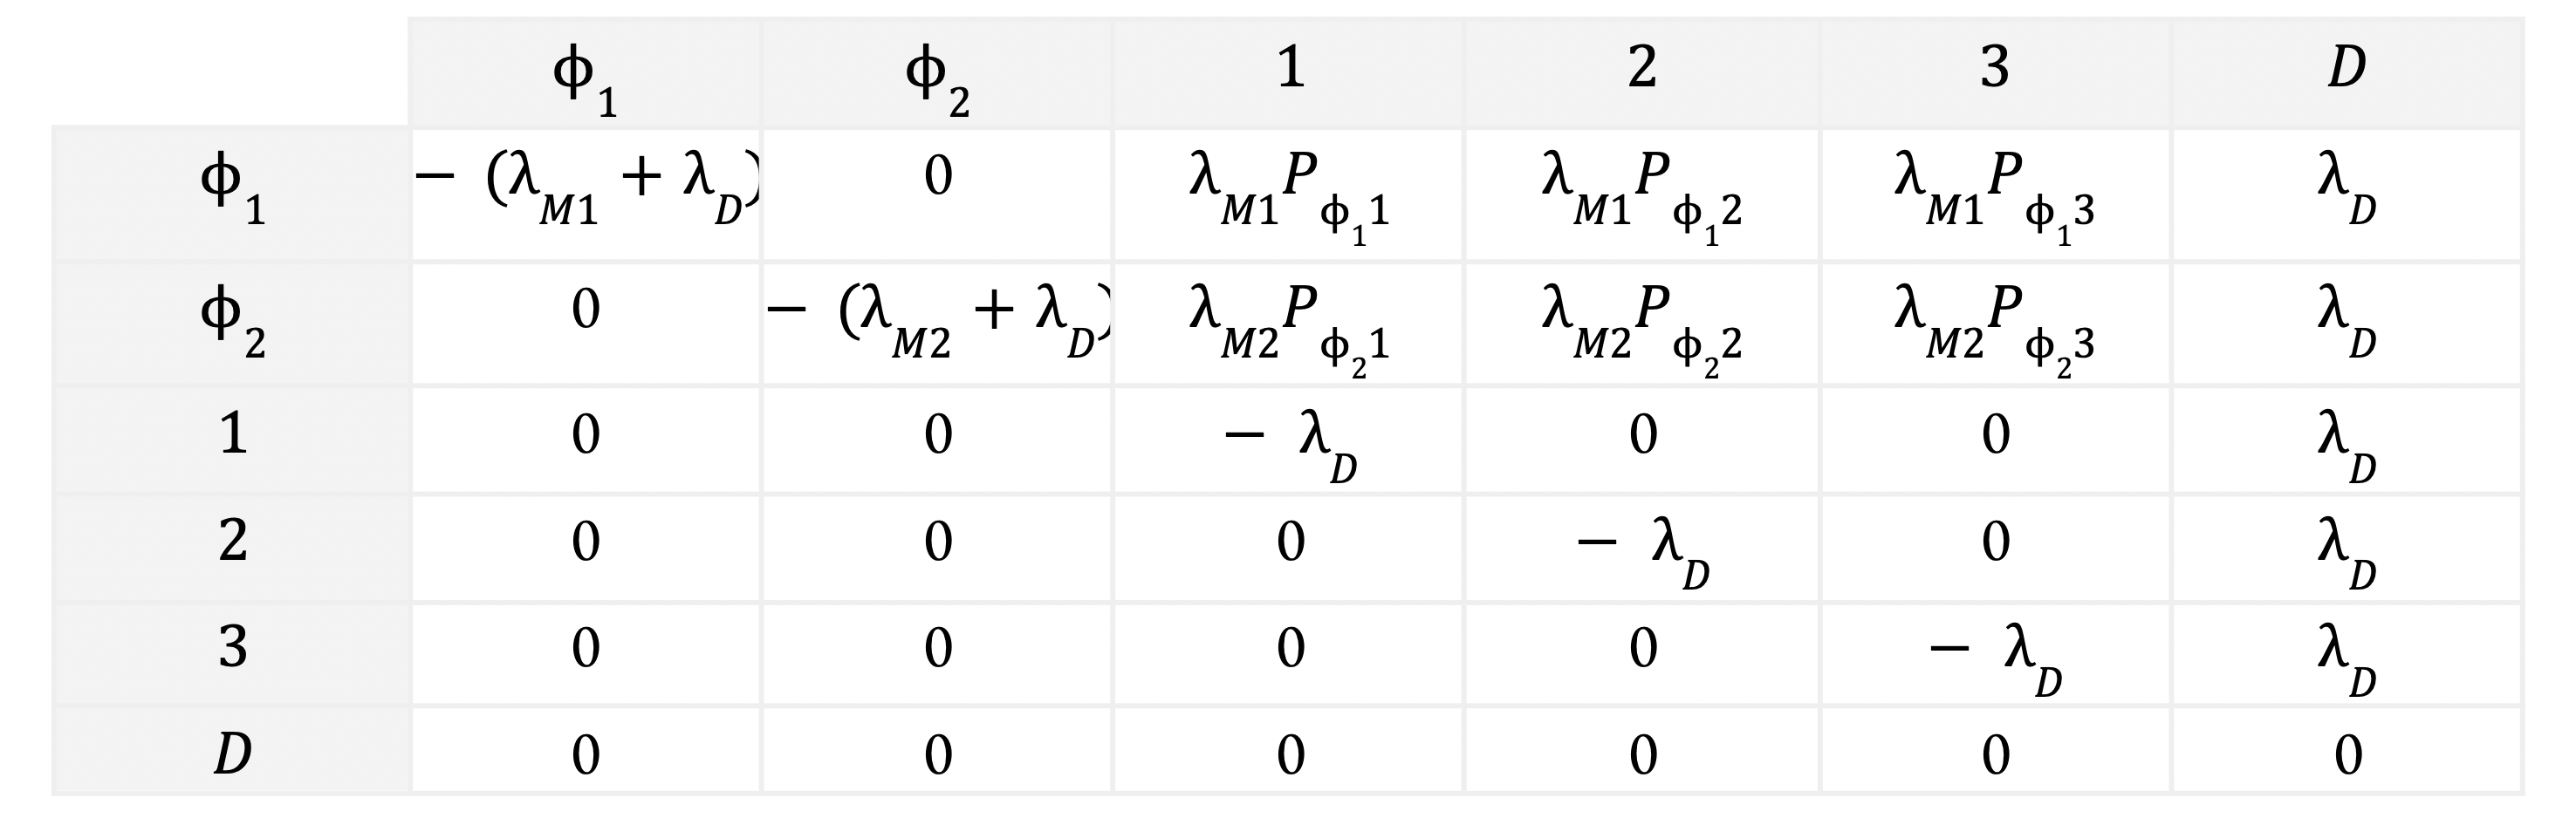
\includegraphics[width=\linewidth]{images/Q.png}
  \caption{Infinitesimal generator $Q$ of toy lineage tracing experiment.  This system containts two target sites $\sigma_1, \sigma_2$ and three potential mutations $1,2,3$. The elements of the infinitesimal generator $Q$ are comprised of the site-specific mutation rates $\lambda_{M \sigma}$, the deletion rate $\lambda_D$, and the indel distrbution $p_{\phi_\sigma s}$. More specifically, $p_{\phi_\sigma s}$ represents the probability transitioning to the observed character state $s$ from some other state $\phi_\sigma$, conditioned on a transition occuring.}
\end{figure}

\subsection*{Log-Likelihood and Triplets Correct for $20$-Cell Simulation}

\begin{figure}[h]
  \label{fig:loss_20}
  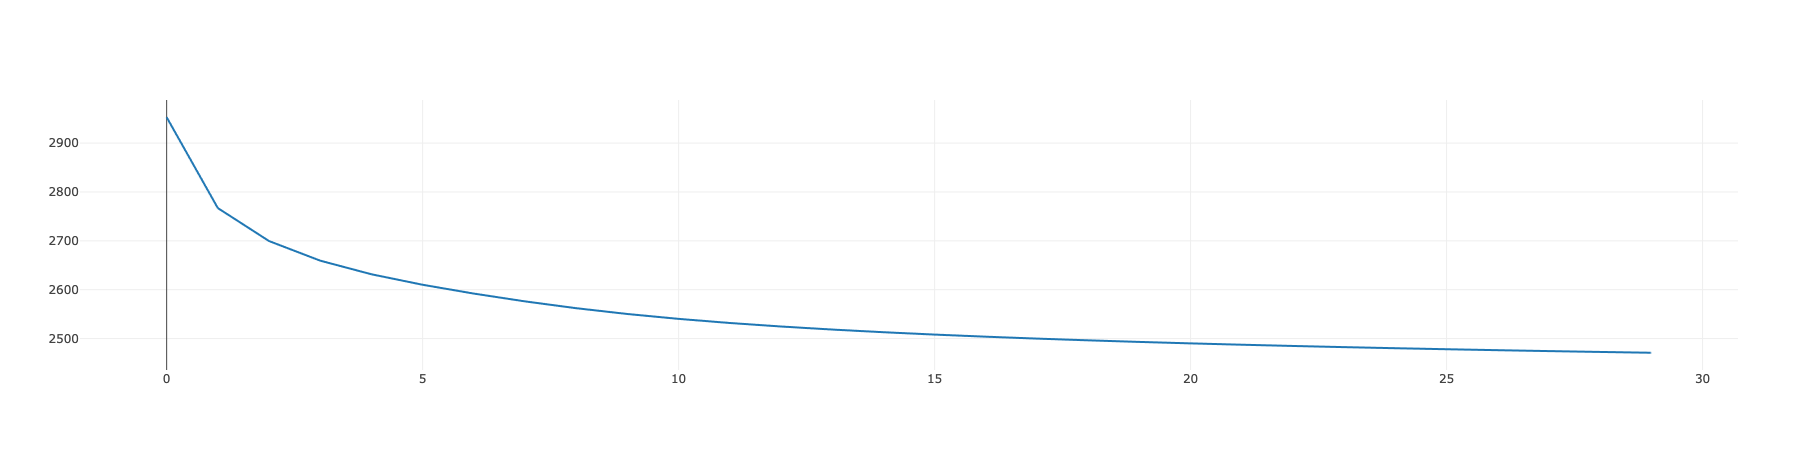
\includegraphics[width=\linewidth]{images/loss_20.png}
  \caption{Epochs on the x-axis and log-likelihood on the y-axis}
\end{figure}

\begin{figure}[h]
  \label{fig:tc_20}
  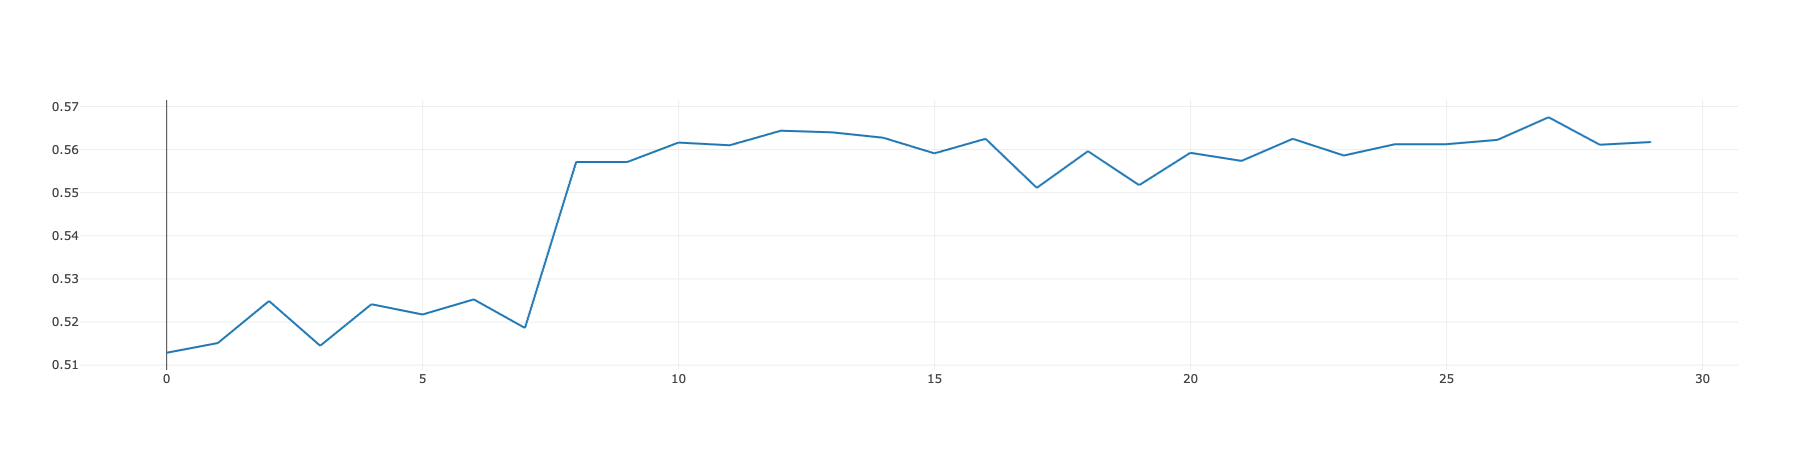
\includegraphics[width=\linewidth]{images/tc_20.png}
  \caption{Epochs on the x-axis and \% triplets correct on the y-axis}
\end{figure}

\clearpage

\subsection*{Log-Likelihood and Triplets Correct for $1000$-Cell Simulation}

\begin{figure}[h]
  \label{fig:loss_1000}
  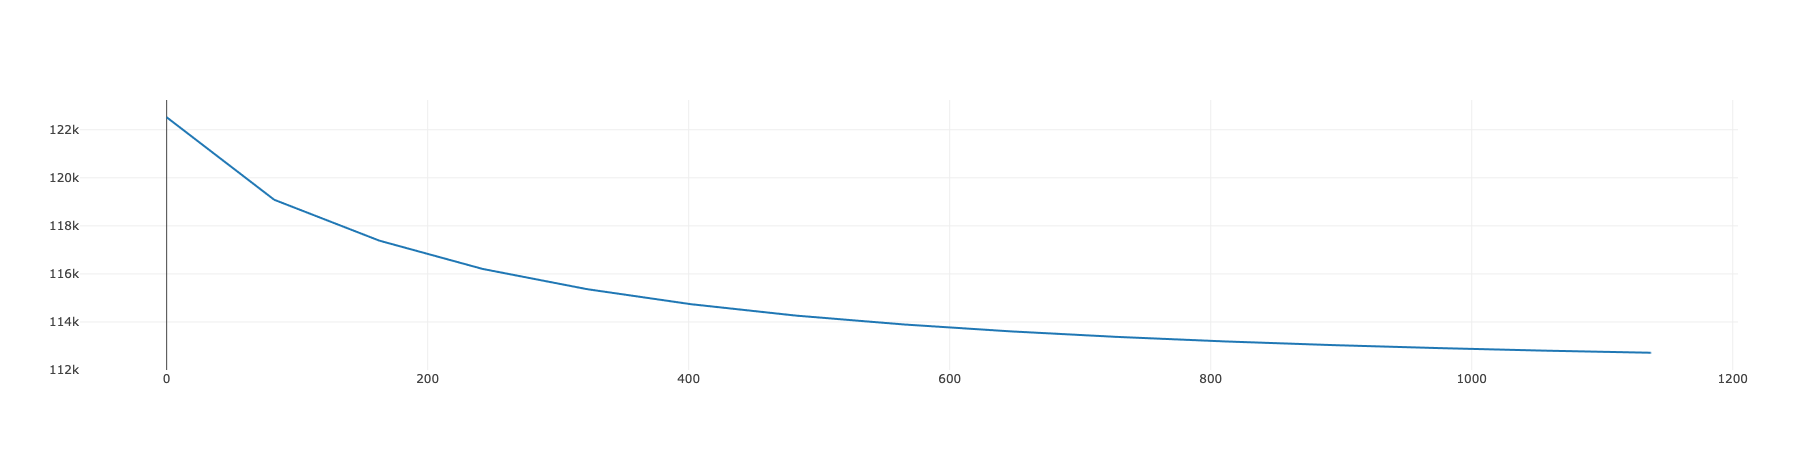
\includegraphics[width=\linewidth]{images/loss_1000.png}
  \caption{Epochs on the x-axis and log-likelihood on the y-axis}
\end{figure}

\begin{figure}[h]
  \label{fig:tc_1000}
  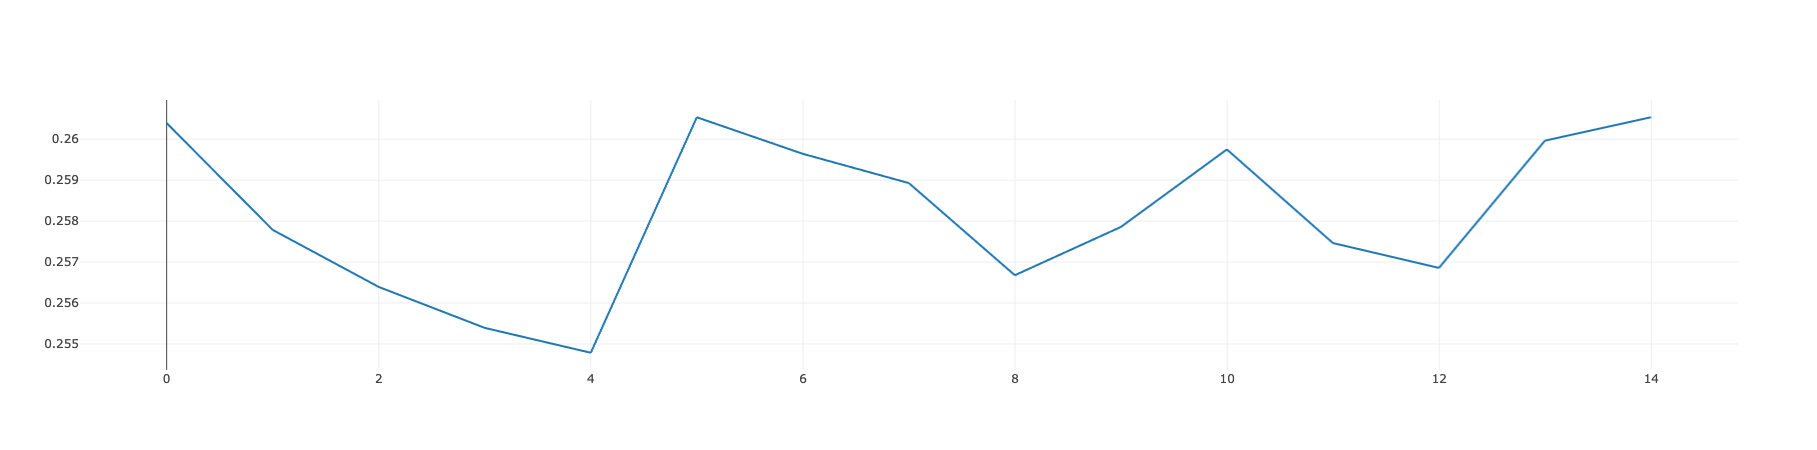
\includegraphics[width=\linewidth]{images/tc_1000.png}
  \caption{Epochs on the x-axis and \% triplets correct on the y-axis}
\end{figure}



\end{document}